\chapter{Flujo de Diseño Digital de Circuitos Integrados con las herramientas de Synopsys. Estructura de Scripting}
\label{ch:scripting}

A continuación se detalla la estructura propuesta para implementar un flujo de diseño de circuitos integrados, y se expone como fueron sometidos los módulos de un microprocesador ASP RISC-V, con el fin de demostrar la efectividad del flujo de diseño digital propuesto. Esta estructura está basada en el manual sobre el uso de las herramientas de Synopsys en el flujo de diseño de ASICs, del Instituto Tecnológico de Costa Rica \cite{FlujoJairo2016}.

La siguiente estructura dista considerablemente de la propuesta en \cite{FlujoJairo2016} y que a su vez está basada en el manual \cite{kommuru2009asic}. En estos trabajos las estructuras se basan en ejemplos simples con diseños \textit{HDL} relativamente pequeños. La siguiente estructura toma como premisa que se trabaja con diseños muy grandes por lo que se requiere de mayor eficiencia en la generación de las bases de datos y archivos necesarios para el diseño.

Dado que las herramientas EDA que se utilizan corren en "Linux", muchos de los scripts que se encuentran en esta estructura, hacen referencia a particularidades de este sistema operativo y no se describen en detalle pues abundar sobre el entorno "CentOS de Linux" esta fuera del objetivo de este proyecto, es por ello que se parte de la premisa que el lector cuenta con el conocimiento suficiente de este sistema operativo.

La primera propuesta de esta estructura fue desarrollada por el Dr. Juan Agustín Rodríguez y se tomó como referencia para desarrollar la que a continuación se expondrá. La estructura que se propone se basa en 3 principios muy relacionados con el mundo de desarrollo de software; sin embargo, apelan más a la experiencia práctica del Dr. Rodríguez y del aspirante que escribió este informe.

\begin{itemize}
\item {\textbf{Regularidad:}} {Este concepto se refiere a la uniformidad con la que los elementos desarrollados se ubican, dentro de la estructura de archivos y directorios, los cuales están basados en un principio o plan.

Esta estructura es "regular" en tanto presenta la misma morfología para los distintos directorios, esto quiere decir que aunque los directorios contienen archivos de distinta naturaleza, la mayoría presentan una jerarquía constante entre sí.}

\item {\textbf{Localidad:}} {Se refiere a usar archivos y directorios únicos, para evitar el manejo de múltiples versiones y múltiples rutas de acceso a archivos que en esencia son iguales, lo cual suele ser un problema cuando se debe involucrar a más personas en un proyecto.

La estructura presenta "localidad" en tanto los archivos fuente y las bases de datos generadas por los procesos de síntesis, únicamente residen en un único directorio y presentan sólo una ruta de acceso, no se generan copias de estos archivos en otros directorios, y la forma en que se accede a ellos es mediante punteros. Existen algunas excepciones a este principio; sin embargo, serán expuestas más adelante y se justificará el porqué de estos archivos.}

\item {\textbf{Continuidad:}} {La "continuidad" hace referencia a dos conceptos, el primero es sobre la capacidad de poder usar elementos en la estructura del flujo para rastrear el diseño en una etapa dada, hasta la etapa de origen que en este caso corresponde al modelo de comportamiento del diseño.

El segundo se relaciona con la capacidad de ser permanente, o en otras palabras tener la capacidad de degradarse con lentitud, es frecuente encontrar que entre diseñadores existan desacuerdos sobre la mejor forma de nombrar los archivos o la mejor manera de ubicarlos y realmente no es posible definir una estructura como la más eficiente o la estructura suprema, pues apela a muchos criterios subjetivos y relativos, tanto por parte de los diseñadores como por la naturaleza de los proyectos. 

Finalmente se afirma que la estructura es continua, ya que la navegación dentro de los directorios permite identificar de forma fácil e intuitiva, las distintas etapas del flujo, y mediante los scripts, y un conocimiento general del flujo descrito en la sección \ref{sec:gen_d_flow}, es posible ubicar los resultados de las distintas etapas y los archivos fuente que se fueron usados para generarlos (los resultados). Respecto a la parte de continuidad en el tiempo, se espera ofrecer una estructura lo suficientemente elegante y práctica para que pueda seguir siendo utilizada en futuros proyectos y que los diseñadores que los enfrenten puedan sentirse cómodos con ella.}

\end{itemize}

\section{Estructura de directorios y archivos}

\begin{figure}[h]
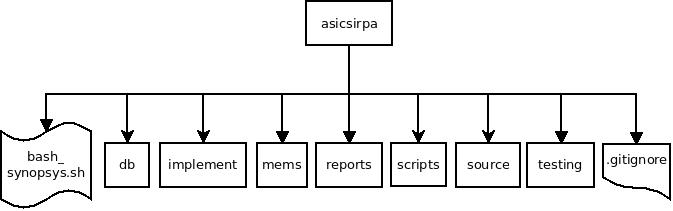
\includegraphics[width=\textwidth]{estructura_1.jpeg}
\centering
\caption{Esquema de la jerarquía de directorios y archivos para implementar el flujo de diseño digital. El archivo .gitignore es un archivo oculto, contiene información para que el sistema de control de versiones opere de forma personalizada, carece de relevancia para la estructura del flujo; sin embargo, permite mantener un repositorio más ordenado. \cite{website:gitignore, website:cvs}}
\label{directorios}
\end{figure}


\begin{figure}[h]
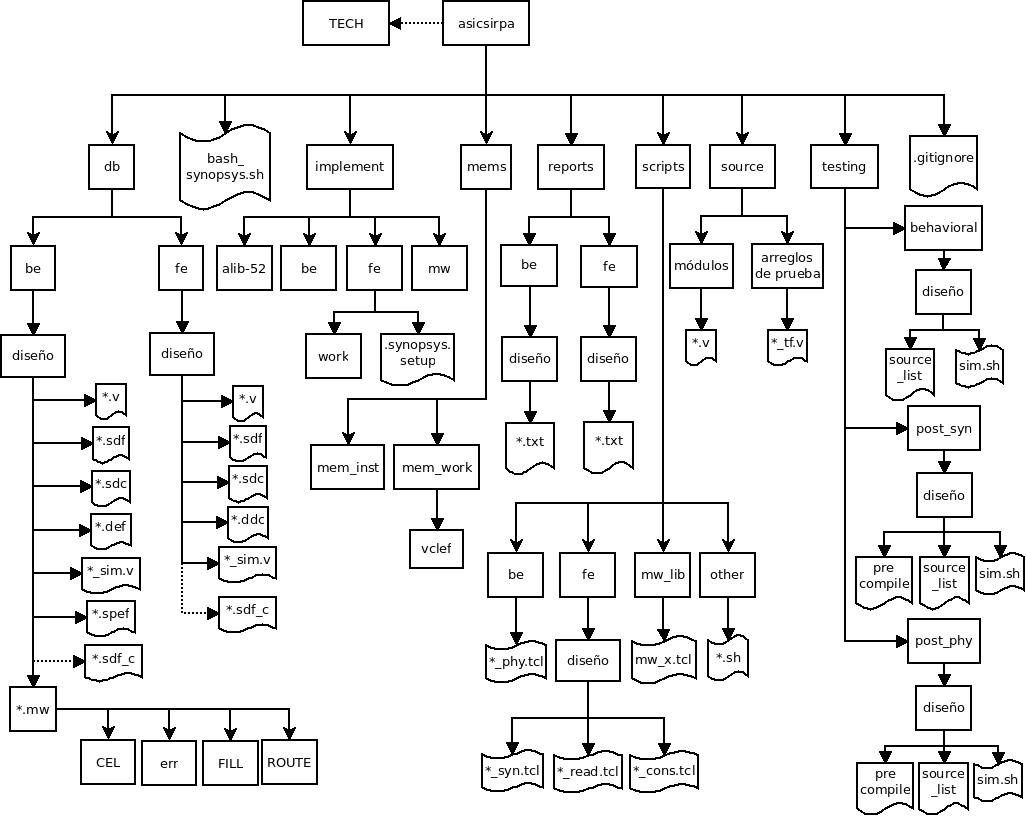
\includegraphics[width=\textwidth]{estructura.jpeg}
\centering
\caption{Esquema completo de la jerarquía de directorios y archivos que implementan el flujo de diseño digital. El bloque \textbf{TECH} hace referencia a la biblioteca de la tecnología, no es buena idea agregar este directorio en la misma ubicación que el proyecto ya que es un directorio de tamaño considerable y copiarlo en cada proyecto representa un mal gasto considerable de memoria, aunque los sistemas modernos tienen una gran capacidad de almacenamiento, siempre es más eficiente manejar únicamente un directorio para la tecnología.}
\label{directorios}
\end{figure}
Como puede apreciarse en la figura \ref{directorios} el directorio base del proyecto contiene hasta el momento siete directorios y dos archivos, uno de los cuales es oculto y carece de relevancia para el proyecto. Comenzando por el archivo \textbf{bash\_synopsys.sh}, tenemos un script de bash, que es una de las tantas consolas que ofrecen los ambientes linux, este script contiene punteros hacia los archivos ejecutables del juego de herramientas de Synopsys, la licencia para que puedan correr, y finalmente cualquier otro software a fín al proyecto pueda ser usado.

Dentro de la estructura propuesta existe un archivo que es importante para que el flujo de diseño sea más cómodo para el usuario, el archivo del que se habla es el archivo \textbf{.bashrc}, el cual es un archivo oculto y se ubica en el directorio principal del usuario, a este directorio suele denominarsele como: "HOME", es universal en cualquier computador con un sistema operativo linux moderno. Este archivo es ejecutado cada vez que se abre una terminal o consola de tipo bash, y le permite al usuario personalizar distintos aspectos de la consola, gracias a esta cualidad es posible abrir una terminal y contar con la posibilidad de disponer de las herramientas necesarias sin tener que ejecutar el script "bash\_synopsys.sh" cada vez que se abre una nueva terminal.

Este archivo (.bashrc) también permite crear variables con rutas relativas a directorios. El contexto en el que se establece la premisa de rutas relativas, corresponde a que el proyecto al ser de dimensiones considerables, involucra a varias personas, y entre otras cosas también existe una herramienta para el manejo de versiones "CVS" \cite{website:cvs}, además es probable que existan muchas copias del proyecto en distintos computadores o servidores.

Así, al hablar de rutas relativas se refiere a que cada computador tiene una ruta absoluta diferente hacia el directorio del proyecto, pero, una vez que se encuentre dentro del directorio del proyecto, las rutas hacia directorios y archivos se vuelven iguales para todos los involucrados. Mediante el uso de variables es posible usar un único comando de referencia en los scripts, y usando variables con rutas relativas, permite abstenerse de editar los scripts en cada computador. Más adelante se expondrá un poco más sobre la importancia de las rutas relativas cuando se hable de los scripts para ejecutar los procesos de síntesis. Podemos ver lo expuesto anteriormente en el diagrama de la figura \ref{bash_syn}.

\begin{figure}[h]
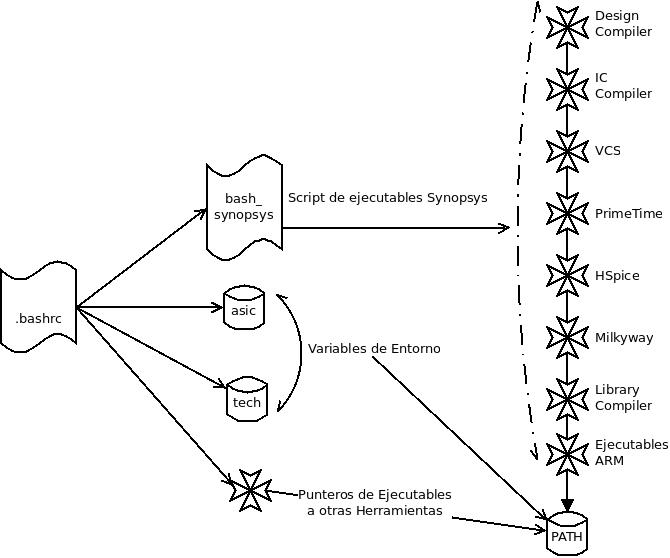
\includegraphics[width=\textwidth]{s_bash.jpeg}
\centering
\caption{Esquema ilustrativo de la relación entre los scripts de bash que inicializan las herramientas EDA y crean las varibles que contienen los punteros a los archivos y la biblioteca de la tecnología de integración}
\label{bash_syn}
\end{figure}

A continuación podemos observar un ejemplo que ilustra, la ejecución del script de bash para incluir en la variable de ambiente "PATH", las rutas a los ejecutables de las herramientas EDA (línea 8), y la creación de 2 variables con la ruta relativa al directorio base del proyecto (variable "asic", línea 3)


\definecolor{mygray}{rgb}{0.5,0.5,0.5}
\definecolor{mygreen}{rgb}{0,0.4,0.1}

\begin{lstlisting}[language=bash, numbers=left, keywordstyle=\color{blue}, commentstyle=\color{mygreen}]
# Home for working on the SiRPA ASIC Integration Project
asic=/home/rcastro/asicsirpa
export asic
# IBM technology files for the Integration Project (Library)
tech=/home/IBM/TECH
export tech
# Load the EDA Synopsys executables
. $asic/bash_synopsys.sh
# Load a text processor application
PATH=$PATH:/home/tools/sublime_text_3
export PATH
\end{lstlisting}


Retomando el diagrama de la figura \ref{directorios}, dentro del directorio del proyecto de integración encontramos siete directorios, de los cuales db, implement, reports y scripts presentan la misma estructura regular, pues en cada uno de estos directorios encontramos otros 2 directorios llamados be y fe, como podrá intuirse hacen referencia a "back end" y "front end" respectivamente, se decidió usar estas abreviaciones por su simplicidad ya que resumen muy concretamente a que hacen referencia y son muy intuitivas.

El directorio \textbf{db} es una abreviación a "Data Base", que en inglés significa base de datos, y precisamente es en este directorio donde se albergan las bases de datos y demás archivos que son producto de los procesos de síntesis, naturalmente en el subdirectorio fe sólo se almacenan los resultados de la sínteisis lógica de los módulos del proyecto.

El directorio \textbf{implement} alude al proceso de ejecución de las herramientas y los procesos de síntesis, este directorio no contiene archivos de gran relevancia para el proyecto, salvo el directorio \textbf{fe} el cual contiene el archivo oculto, \textbf{.synopsys\_dc.setup}, que es un script de \textit{TCL} con comandos de inicialización y preconfiguración de la herramienta \textit{Design Compiler}, este script es de vital importancia para que la herramienta opere de forma adecuada, más adelante se expondrá un poco más sobre este archivo. Este directorio se emplea para concentrar los archivos temporales que se producen cuando se trabaja con las herramientas de síntesis, los directorios \textbf{work} en fe, el cual contiene archivos que se generan al analizar el código fuente en \textit{HDL}, el directorio \textbf{alib-52} que contiene las bibliotecas producto de la compilación del diseño, esta biblioteca contiene información de caracterización de la biblioteca de la tecnología y sirve para acelerar compilaciones subsecuentes. Finalmente dentro del directorio \textbf{implement} tenemos otro directorio llamado \textbf{mw}, este directorio contiene los reportes y anotaciones de la ejecución de la herramienta \textit{Milkyway}, que es una herramienta de \textit{back end} y podría incluirse en el directorio \textbf{be}; sin embargo, se considera adecuado que esta herramienta tenga un directorio particular para sí, más adelante se explicará la funcionalidad de esta aplicación y el porqué de esta separación.

Siguiendo con los directorios que presentan regularidad, encontramos los directorios: \textbf{reports} y \textbf{scripts}, los cuales contienen reportes y scripts respectivamente. Los reportes generados son distintos de los que genera la herramienta a la hora de estar haciendo el proceso de síntesis, estos reportes corresponden a la información final de síntesis y proveen información útil en la toma de decisiones de las etapas posteriores. Luego los scripts, son los códigos principalmente en lenguaje \textit{TCL} donde se condensan los comandos que usan las herramientas para generar los procesos de síntesis. En el directorio scripts se observan otros dos directorios, \textbf{mw} y \textbf{other}, que contienen respectivamente contienen scripts para la herramienta \textit{Milkyway}, y de otras herramientas como por ejemplo \textit{MATLAB} y los generadores de memorias \textit{SRAM} de \textit{ARM}, los cuales serán expuestos más adelante.

Los tres directorios restantes, \textbf{mems}, \textbf{source}, y \textbf{testing}, no presentan una estructura regular como la que hemos visto hasta el momento, el directorio \textbf{testing} podría incluirse en esa categoría; sin embargo, la subdivisión que presenta es bastante puntual e intuitiva, así que se considera más práctica. Como se puede abstraer "testing", es una palabra en inglés cuya traducción es "pruebas", aquí se alojan los resultados de las distintas simulaciones con las que se valida la funcionalidad de los módulos sometidos al flujo, las simulaciones se subdividen en tres categorías, por comportamiento, en inglés, \textbf{behavioral}, post síntesis lógica (\textbf{post\_syn}), y post síntesis física (\textbf{post\_phy}). Estos tres directorios cuentan con 3 archivos principales, los punteros de compilación, archivos fuente, y un script en \textit{bash} que permiten invocar la herramienta de simulación y ejecutar las compilaciones y simulaciones respectivas, luego de la simulación puede que sea de interés guardar un vector de resultados en un archivo de texto. Así que los directorios de simulación presentan cuatro archivos importantes, los archivos extra que puedan encontrarse en estos directorios son producto de los apuntes y registros que genera la herramienta durante la compilación, y pueden ser obviados.

El directorio \textbf{source}, que se traduce como fuente, contiene dos categorías de directorios, el primero corresponde a los archivos \textit{HDL} con la información modular del diseño, es decir los archivos con la descripción por comportamiento del diseño, y también los archivos con los vectores de estimulos y arreglos o bancos de prueba, es decir los \textit{testbenchs o testfixtures}. Los primeros usados en el proceso de síntesis lógica, y los últimos necesarios para las simulaciones en los distintos dominios.

Por último tenemos el directorio \textbf{mems}, el cual es un directorio bastante particular. Contiene la información producida por los aceleradores de diseño de \textit{ARM}, los cuales generan celdas de memoria \textit{SRAM}. Se trata este proceso aparte ya que los programas para generar las celdas de memoria tienen una metodología de trabajo un poco diferente de la del flujo digital que se ha venido exponiendo. La justificación de manejar estos directorios aparte recae en no mezclar las metodologías de trabajo; sin embargo, el producto final de este procedimiento se integra a la estructura que se ha venido describiendo, es decir se generan bases de datos para las etapas de \textit {back y front end}, posteriormente se ahondará en detalles cuando se expongan los scripts de síntesis de las \textit{SRAM}.

En este directorio (\textbf{mems}), se encuentran dos directorios principales, \textbf{mem\_inst}, el cual contiene los ejecutables de las herramientas de \textit{ARM} para sintetizar las memorias, es importante que sólo exista una única copia de este directorio, ya que es muy pesado (en términos de espacio, cerca de 2 GB), y generaría saturación en un repositorio, que se debe mantener simple y con la menor densidad posible. El otro directorio es \textbf{mem\_work}, el cual contiene el resultado de la síntesis de las celdas \textit{SRAM} y finalmente \textbf{vclef} el cual es un archivo con la información de los metales y el enrutado de la celda \textbf{SRAM} física, este último se crea con el fin de facilitar la ejecución de la herramienta \textit{Milkyway} y generar las base de datos necesarias para los procesos de \textit{back end}. Nuevamente esto será discutido en detalle en un apartado posterior.



\section{Scripts de Front End}
\label{sec:syn_s}
\subsection{Script de síntesis lógica}
\label{script_syn}
En la figura \ref{s_syn} se observa como la síntesis lógica se ejecuta mediante tres scripts, dos de los cuales son auxiliares al script de síntesis, los scripts se nombran de acuerdo con un nombre representativo del diseño con el que se trabaja, aunque suele ser conveniente nombrar los archivos de la misma manera al módulo principal, si este nombre es muy largo, es preferible optar por un nombre representativo.

\begin{figure}[h]
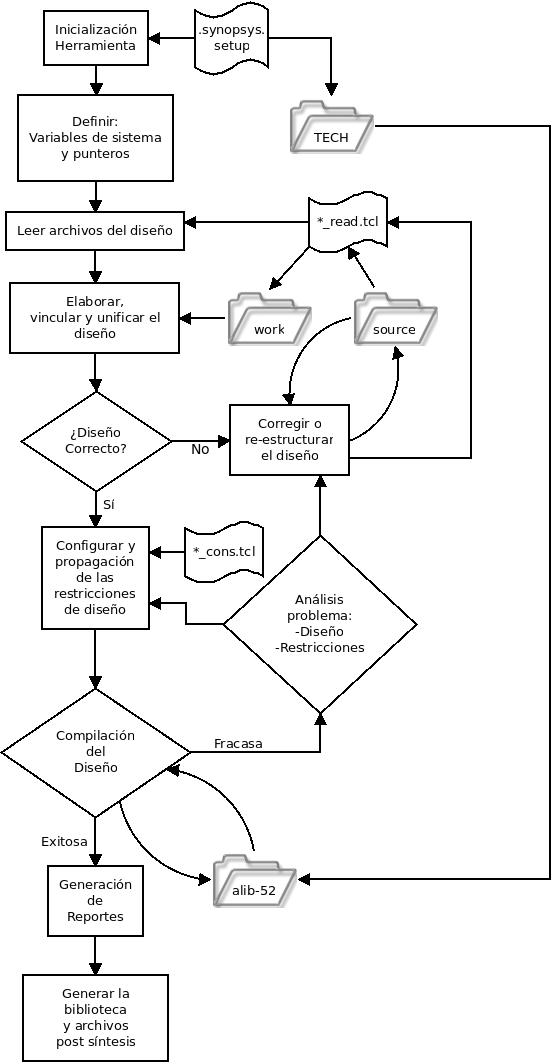
\includegraphics[scale=0.55]{log_syn.jpeg}
\centering
\caption{Diagrama de flujo del scripting que ejecuta la síntesis lógica}
\label{s_syn}
\end{figure}



Es aconsejable separar las instrucciones de síntesis de la herramienta para no generar scripts densos en código y modular las operaciones ejecutadas por la herramienta.

Existe un único flujo en la ejecución de los scripts. El script principal, (*\_syn.tcl) contempla el diagrama de la figura \ref{s_syn}, a partir de la etapa en la que se definen los punteros y las variables del sistema, continúa en línea recta hasta la generación de la base de datos y demás archivos post síntesis. En un apartado anterior se mencionó sobre la importancia del script \textbf{.synopsys\_dc.setup}, este archivo contiene comandos y procedimientos de \textit{TCL} que ejecutan tareas configuración, tal como inicialización de parámetros y variables, declaración de las bibliotecas de diseño.

Cuando la herramienta \textit{Design Compiler} es invocada, ésta busca el archivo configuración en la dirección desde dónde fue invocada, al leer los archivos la herramienta tendrá la información de la ruta hacia las bibliotecas, y cualquier otra personalización que el usuario considere necesaria para facilitar el uso de la herramienta, como crear un alias para comandos en particular, definir la ruta del directorio \textit{alib-52}, el cual se usa para sintetizar una biblioteca reducida y acelerar el proceso de compilación lógica, aunque este es un directorio que le facilita la operación a la herramienta, y las bibliotecas generadas pueden ser utilizadas en etapas posteriores del diseño, no es imperativo que este directorio permanezca en el proyecto, y tampoco es imperativo incluirlo en un repositorio, ya que versionarlo carece de sentido práctico.

Otro de los usos más significativos que se le da al archivo \textbf{.synopsys\_dc.setup} en este proyecto es adquirir variables del sistema operativo para definir variables locales al entorno de la herramienta, estas consisten consiste en rutas relativas al directorio base del proyecto y el directorio base de la biblioteca de la tecnología.

Crear este tipo de variables facilita que los scripts puedan parametrizarse y estos sean capaces de ser usados en distintos equipos sin tener que alterarlos o acondicionarlos significativamente, para que puedan ser funcionales independiente a las rutas locales de los archivos en otros equipos.

Cabe destacar que no toda la configuración de parámetros y variables se realiza en este archivo, y aunque es posible, tampoco es eficiente hacerlo. Este archivo tiene un caráter más genérico. Su función es poner la herramienta a punto para que este en capacidad de sintetizar correctamente cualquier diseño. Las particularidades de los diseños que se trabajan son contempladas en el script de restricciones (constraints), así que no todas las restricciones de diseño se incluyen en este script, sólo las que son universales para cualquier diseño. 

Una vez que la herramienta ha sido inicializada, se procede a configurar variables y parámetros propios del diseño con el que se trabaja. Estos son principalmente variables de rutas hacia el destino de los archivos de salida, y reportes, así como punteros hacia la ruta a bibliotecas auxiliares para el diseño en particular. Así también se crean variables con el nombre del proyecto para que al generar los archivos de salida se usen los comandos de forma paramétrica. Es decir los comandos dependen del valor o contenido de las varibles, esto último se realiza con la finalidad de tener un script genérico, al cual se le deba dar una edición mínima cuando deba ser adaptado a otro diseño.

\subsubsection{Script de lectura de archivos fuente}

Cuando finalmente se han definido todos los parámetros y variables generales para el diseño particular con el que se trabajará, se procede a leer los archivos fuente del diseño, esto corresponde a los módulos descritos en \textit{HDL}. El conjunto de estos archivos \textit{HDL} suelen denominarse como diseño descrito en \textbf{RTL}\footnote{RTL, refiere a Register Transfer Level. Su traducción corresponde a nivel de transferencia mediante registros, dentro del argot del diseño VLSI refiere a la metodología con la cual se describe un dispositivo digital usando un lenguaje de alto nivel, cuya semántica concuerda con el comportamiento del dispositivo digital.} La herramienta debe analizar cada archivo, dependiendo del proyecto pueden existir una enorme cantidad de módulos por analizar, esta es la razón por la que se genera un script de lectura de módulos.

Usando las ventajas de los lenguajes compilados como lo es \textit{TCL}, la lectura y análisis de los módulos se puede realizar de forma programática. En el script \textbf{*\_read.tcl} se usa una variable con el puntero hacia el directorio base de los archivos \textit{HDL} fuente, luego mediante una subrutina de \textit{TCL} se crea una colección con los directorios que contienen los distintos módulos posteriormente se ejecuta un pequeño algoritmo recursivo que recorre las colección de los directorios, para cada directorio se crea otra colección con los módulos, los cuales nuevamente son leídos de manera recursiva. Al recorrer esta última colección se ejecuta el comando de análisis de la herramienta, así se analizan todos los módulos del diseño de forma automática, sin tener la necesidad de incluir en el script la misma instrucción repetida para leer cada posible archivo del proyecto.

\begin{figure}[h]
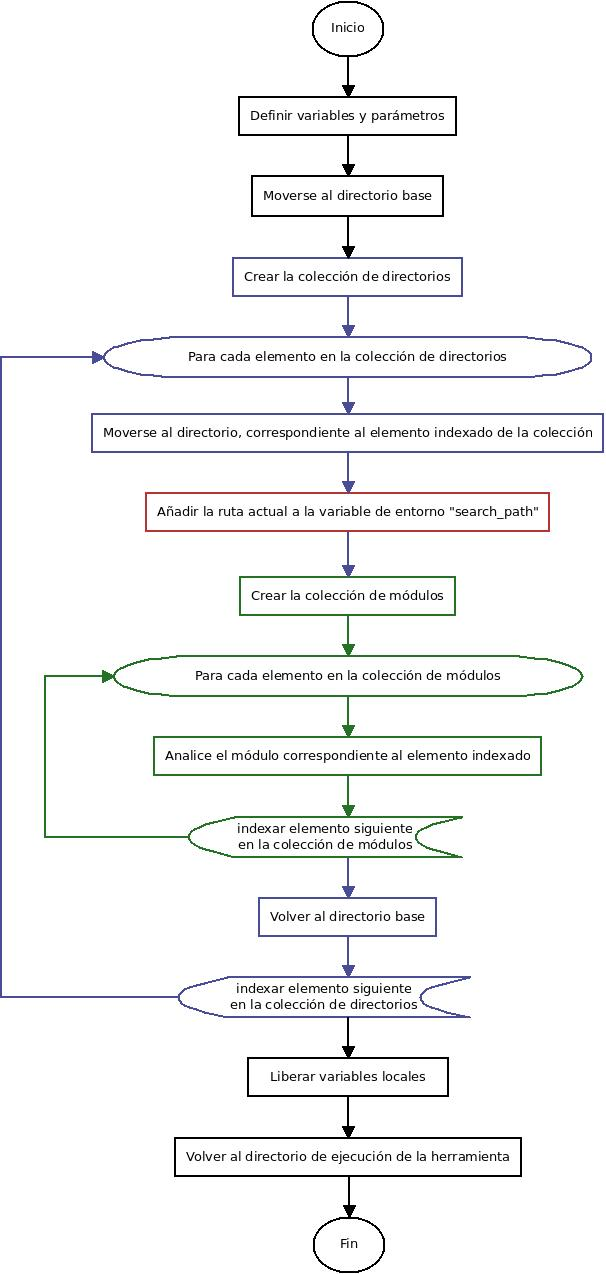
\includegraphics[scale=0.45]{read_script.jpeg}
\centering
\caption{Algoritmo recursivo de lectura y análisis de los módulos \textit{HDL} del diseño}
\label{s_read}
\end{figure}

En la figura \ref{s_read} se observa un diagrama de flujo, con el resumen gráfico del algoritmo descrito en los párrafos anteriores, cabe destacar que en el bloque que indica la definición de variables y parámetros hace referencia a variables locales para ejecutar las tareas de lectura, aunque en realidad únicamente se crean punteros (a los que también llamaremos variables de ruta) hacia las rutas base de los archivos fuente.

Cabe destacar que para algunos diseños, las variables de ruta no necesariamente apuntan a directorios con contenido \textit{HDL}, pues como suele hacerse en proyectos muy grandes, conviene dividir el diseño general en subdiseños más compactos, esto último implica que para algunos proyectos es preferible leer las bases de datos generadas para otros diseños, pues es más práctico.

Otra observación que se debe realizar al diagrama de la figura \ref{s_read} es que no en todos los diseños es necesario crear una colección de directorios, pues si todos los archivos fuente de ese diseño se concentran en un directorio, recorrer la colección de directorios carece de sentido. Consecuentemente puede omitirse el lazo de color púrpura, correspondiente al algoritmo iterativo de indexación de directorios. El único lazo estrictamente necesario para leer los archivos fuente, es el lazo en color verde. Se incluyen ambos lazos en la figura \ref{s_read}, y se expuso el proceso de lectura y análisis con los dos lazos para ilustrar el caso más general de lectura de archivos fuente. Naturalmente los scripts deben ajustarse a la estructura particular del diseño; sin embargo, el algoritmo expuesto es fácilmente adaptable a cada caso.

Siguiendo con la figura \ref{s_read}, y dándole continuidad a la idea expuesta en el párrafo anterior,procede declarar que conviene conservar el bloque de añadir en la variable "search\_path" la ruta actual (bloque en color rojo), ya que al usar el comando de análisis de la herramienta \textit{Design Compiler}, si la ruta relativa al archivo no se ha incluído a la variable de búsqueda (search\_path) la herramienta ofrecerá un error, pues se pretende acceder a una ubicación que no ha sido autorizada para la herramienta.

La variable "search\_path", es una variable propia del entorno de las herramientas de \textit{Synopsys}, su función es manejar una colección de ubicaciones o rutas permitidas para que le herramienta pueda leer y escribir archivos.

Finalmente conviene volver a la ubicación desde donde se ejecutó la herramienta para evitar crear archivos de apuntes, o archivos temporales con poca relevancia para el proyecto, en directorios ajenos a los destinados para esta tarea. Basta decir que liberar todas las variables locales al finalizar una subrutina es una buena práctica de programación, así que es conveniente hacerlo.

Volviendo a la ejecución del script principal de síntesis, cuando ya todos lo módulos son leídos, en el directorio work se crean archivos con información sobre el resultado del análisis de los módulos, de momento estos archivos serán fundamentales para avanzar en el flujo de síntesis, pero una vez acabado el flujo y habiendo generado la base de datos del diseño, no son tan relevantes.


Dicho lo anterior, se debe proceder a elaborar el diseño, esto consiste en definirle a la herramienta cuál es el módulo principal del diseño, posteriormente se deben vincular y unificar todos los módulos. La vinculación y unificación establece la jerarquía modular del diseño y resuelve la interdependencia de los módulos.

En la figura \ref{s_syn} se observa un bloque condicional (diamante de decisión), evaluando la condición si el diseño es correcto. En otras palabras, la herramienta evalúa entre otras cosas, si la semántica del código es correcta, no existen errores sintácticos y todas las dependencias se cumplen. Este bloque condicional no se asocia a una subrutina programática en el script, de hecho ninguno de los bloques condicionales que se aprecian en este diagrama lo hace, en la semántica del flujo también interviene el criterio del diseñador y este es un claro ejemplo de esta situación.

Muy probablemente cuando se le solicite a la herramienta evaluar el diseño, aparecerán mensajes de información, alarmas, y en el peor de los casos, errores. El diseñador entonces, deberá evaluar el escenario con el que se enfrenta, corregir los errores es imperativo; sin embargo, muchos de las alertas son tolerables o inofensivas, así que de acuerdo con la experiencia del diseñador se deberá mejorar o no el diseño, y solucionar o aprobar los mensajes de alerta. ¡Un ingeniero en diseño VLSI, debe aprender a vivir bajo el warning!


Si el diseñador no se siente satisfecho con el resultado de la comprobación de la herramienta, y los mensajes sugieren que debe hacer correcciones a los archivos fuente del diseño, lo más sensato es ponerse en contacto con el departamento o personal encargado del diseño por comportamiento y exponer la situación. En algunos casos el diseñador de \textit{front end} podrá verse arrastrado a analizar y corregir el código fuente, esto suele ser muy raro, ya que las tareas en el flujo de integración suelen estar muy bien definidas de acuerdo con departamentos creados para delimitar y definir tareas y responsabilidades, al menos es así en las industrias de gran envergadura; sin embargo, para diseños de baja envergadura, e instituciones académicas es común encontrar a una única persona realizando todas las tareas relacionadas al flujo.

Cuando la comprobación del diseño es aprobada, lo siguiente es establecer las cotas del comportamiento o dicho de otro modo, las restricciones de operación del diseño y propagarlas por la jerarquía, así todas las dependencias tendrán las mismas condiciones de funcionamiento . Esto quiere decir que se deben definir las condiciones bajo las que el diseño va a operar, como por ejemplo, se definen las características de señales críticas y de alta importancia para el diseño como el reloj.

\subsubsection{Script de restricciones}

En esta etapa es donde se invoca el script de restricciones, en inglés "constraints". Este script se encuentra en el flujo del diagrama de la figura \ref{s_syn} como \textit{*\_cons.tcl}. Para este script no hace falta mostrar un diagrama de flujo sobre su comportamiento ya que en principio sólo define parámetros y variables de entorno de la herramienta \textit{Design Compiler}.

A continuación se presenta un pequeño resumen de los parámetros que se consideran suficientes para cumplir a cabalidad las expectativas de desempeño del diseño.

\begin{itemize}
\item \textbf{Señal de reloj:} {Esta señal necesita en principio ser creada, con esto se refiere a generar un objeto\footnote{Entendiendo por objeto al concepto de programación de alto nivel asociado al ente programático capaz de presentar una colección de atributos y permitirle a funciones complejas invocarle y utilizar sus atributos en tareas específicas. Para más información se invita al lector a que consulte un diccionario sobre terminología en el diseño de software} para que la herramienta pueda crear un árbol de reloj hacia los módulos sincrónicos del diseño. Debe definirse un nombre representativo para la señal en el diseño, hay que recalcar que es conveniente definir una nomenclatura estándar para un proyecto grande que involucre diseños jerarquizados, así cada subdiseño tendrá una señal de reloj con las mismas propiedades y un mismo nombre.

Una vez se crea el objeto "señal de reloj", se definen sus propiedades, en esencia, se define el periodo, la incertidumbre, el sesgo y la latencia de la señal, siempre asociando cada propiedad al objeto "señal de reloj" que ha sido creado. Pueden definirse más propiedades, o las mismas de una forma diferente, ya que la herramienta lo permite, pero se considera que estas son suficientes.}

\item \textbf{Propagación de señales:} {Cuando se tienen señales universales a todos los módulos secuenciales, como lo suelen ser las señales de reloj, reset (reinicio), enable (habilitación), preset (preconfiguración), etc. Es posible y es conveniente definir condiciones de comportamiento para la herramienta, ya que esta suele hacer cosas indeseables como colocar buffers en el camino de propagación de señales críticas. Una compuerta lógica, como lo es un buffer presentará efectos de retardo de propagación, lo cual a posteriori se traduce en problemas de sincronización. Es por ello que para estas señales se define un atributo para que la herramienta no realice optimizaciones en ellas. Y el diseñador tendrá un mejor control sobre lo que suceda con esas señales. En este caso únicamente la señal de reloj y reset se definen como intocables.}

\item \textbf{Comportamiento de otras señales:} {Para generar de forma adecuada los modelos simulación, y hacer estimaciones certeras sobre la sincronización de las señales, es beneficioso definir los retardos de propagación de entrada y salida de todas las señales, excepto las mencionadas anteriormente (reloj y reset). Los estímulos en el cableado no se propagan de forma inmediata, por lo que se debe procurar emular un comportamiento cercano a la realidad, para que el resultado de la síntesis del diseño sea lo más confiable posible.}

\item \textbf{Modelo de carga para el cableado:} {Continuando con la idea de generar un modelo lo más realista posible, se deben considerar las características energéticas del cableado.

Conocer las parasitancias de los materiales que se pretenden usar para alimentar e interconectar los módulos del diseño, permite elaborar modelos de comportamiento más cercanos a la realidad. Conocer las propiedades resistivas ayuda a elaborar estimaciones de consumo y desempeño energético, los efectos capacitivos e inductivos permiten evaluar los fenómenos de retardo en las señales, consumo de potencia dinámica, cuando hay conmutación en las señales. Incluso, es posible considerar interferencia por radiación de campos eléctricos y en menor medida los magnéticos. Conocer el área que el enrutado ocupará también es importante para que la herramienta genere una buena optimización del colocado y el enrutamiento. El modelo de cableado o alambrado, es fundamental en sistemas de integración modernos, donde la escala de integración es cada vez más pequeña, a partir de los 300 nm es imperativo contemplar estos efectos.}

\item \textbf{Celdas de conducción:} {El nombre de este atributo, es "driving\_cell", la traducción literal al español no es muy certera; sin embargo, es suficientemente clara. La herramienta necesita que este atributo sea definido para usar una celda adecuada, un buffer, para conectar los módulos del diseño a los puertos de entrada y salida. Esto debe hacerse, en las señales que se propagan hacia puertos de entrada y salida principales e intermodulares.

Una carga excesiva para las señales, suele asociarse a pérdida de información, e inclusive inoperabilidad de algunos segmentos, no se entrará en detalles sobre porqué es importante respetar los fanouts\footnote{El fanout o abanico de salida hace referencia a la máxima cantidad de carga (conexiones) que una señal o puerto es capaz de manejar, hasta que por razones de potencia, esta se empiece a degradar y la señal alcanza niveles de tensión que pueden conducir a la metaestabilidad.} de las señales.

Contemplar las capacidades de conexión de una señal hacia múltiples dependencias, y garantizar la integridad de la información transmitida por dicha señal, es una práctica muy favorable para garantizar la operación exitosa de un diseño. Es por ello que en este apartado también se define un valor máximo de fanout}

\item \textbf{Factor de Actividad:} {El factor de actividad es un parámetro que le indica a la herramienta, como promediar el consumo de potencia dinámico de las señales. En la literatura este parámetro se denomina con la letra griega alfa (\textbf{$\alpha$}).

El factor de actividad, $\alpha$, indica cuantas veces conmuta una señal por ciclo de reloj, naturalmente en un diseño complejo habrán muchas señales con factores de actividad diversos y este cambiará de acuerdo con la tarea que se ejecuta. El valor adecuado a usar en este parámetro responde más a la evidencia empírica y a la experiencia del diseñador.\cite{book:weste2005}

El uso de este parámetro ofrece la posibilidad de generar un reporte de estimación de consumo energético más cercano al comportamiento real del diseño.}
\end{itemize}

Existen muchos otros parámetros que permiten personalizar y condicionar de forma más profunda el diseño, no obstante se expusieron las principales categorías que se deben contemplar y algunas particularidades que se consideran importantes para generar modelos suficientemente cercanos a la realidad. La selección de parámetros suele ser hecha por los ingenieros que se definen los alcances y el desempeño esperado del diseño.

Una vez que las restricciones de diseño han sido definidas y propagadas. Se procede a compilar el diseño, que es la esencia de la síntesis lógica. La compilación le indica a la herramienta que debe generar un nuevo proyecto usando las celdas estándar de la biblioteca de la tecnología, e implementar la estructura abstraída del modelo por comportamiento analizado. En resumen a partir del resultado del análisis del diseño en \textit{HDL} se crea una nueva estructura que mantiene la jerarquía de las funciones y tareas, pero estas ya no se implementan mediante código \textit{HDL} si no mediante elementos de circuitos digitales. En la figura \ref{comp} se observa una analogía gráfica de lo expuesto anteriormente.

\begin{figure}[h]
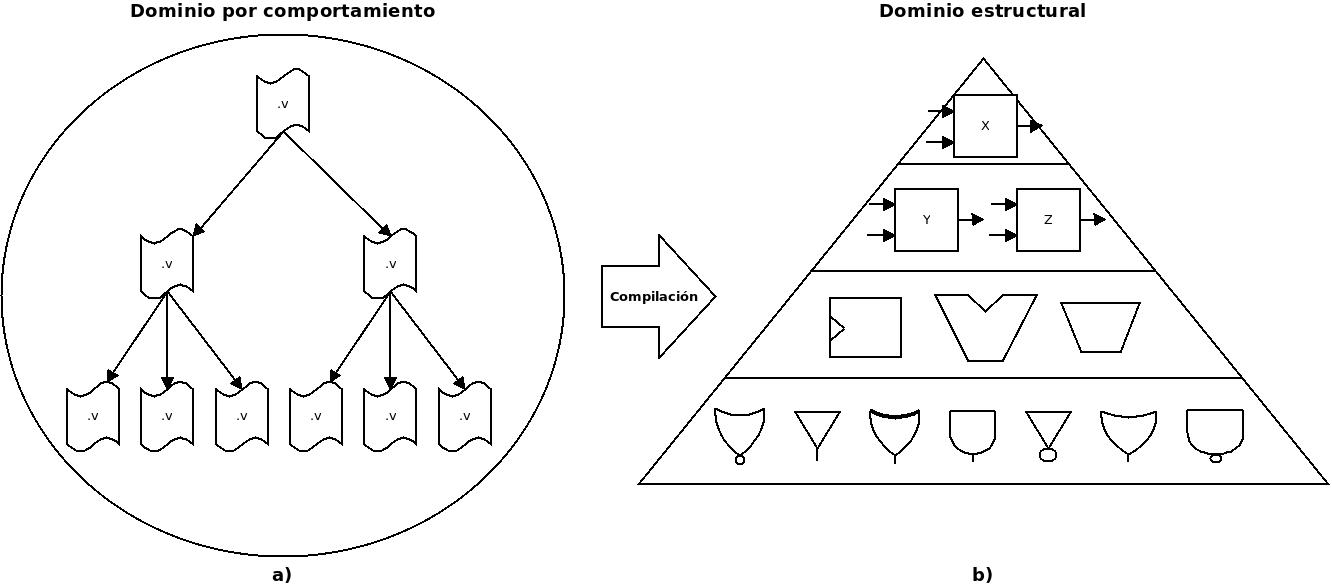
\includegraphics[width=\textwidth]{Compile.jpeg}
\centering
\caption{Ilustración del proceso de compilación. En figura \textbf{$a)$} se aprecia la estructura jerárquica de códigos en \textit{HDL}, y en la figura \textbf{$b)$} la jerarquía abstraída, implementada mediante distintos niveles de elementos digitales, pasando desde funciones complejas, módulos digitales avanzados, hasta compuertas lógicas fundamentales.}
\label{comp}
\end{figure}

Retomando la figura \ref{s_syn} recordamos que el bloque de compilación nuevamente es representado por un diamante de decisión, este diamante no refiere a un evento programático, si no a una etapa en la que el diseñador deberá evaluar si la compilación del diseño es satisfactoria. En esencia la compilación se corrobora mediante la solicitud de reportes a la herramienta, en este punto las bibliotecas compiladas en el directorio \textit{alib-52} y los alias creados en el script de inicialización son bastante útiles, ya que es posible repetir el procedimiento de compilación con relativa facilidad y rapidez.

Es conveniente desviar los resultados de la síntesis (compilación) hacia archivos, para mantener un registro. Esto permite llevar un registro del comportamiento de los diseños, y en caso de que se deba se podrá consultar el resultado de un proyecto anterior, para así evaluar si de ser necesario incluirlo en otro proyecto, ese proyecto anterior cumple las expectativas para el nuevo diseño.

La herramienta permite generar reportes de:

\begin{itemize}
\item \textbf{Sincronización (timing):} {Consiste principalmente en la tabulación de la información asociada a la propagación de la señal de reloj del circuito. Es un análisis que estima el retardo en el diseño basándose únicamente en la topología de las rutas de propagación de la señal de reloj.

A lo anterior se le conoce como \textbf{esfuerzo lógico}, por lo tanto la solicitud de este reporte a la herramienta, consigue un analisis de esfuerzo lógico en el diseño. La herramienta genera entonces un presupuesto teórico de cuanto debe tomarle a la señal, el propagarse a través de una determinada ruta, y evaluar, junto con la información suministrada por las restricciones del diseñador, y la información que aporta la biblioteca de la tecnología, si los datos llegan en el tiempo presupuestado, conocido como "slack MET"\footnote{Es posible ahondar más sobre qué es el "slack" y cual es su relevancia; sin embargo, este informe pretende desvelar el flujo de diseño digital. Se parte de la premisa que el lector comprende el uso de términos como: slack, hold time o setup time, hablar más al respecto está fuera del objetivo de este informe.}.}

\item \textbf{Potencia:} {Se refiere a una descripción resumida de las características de alimentación del diseño, esto se refiere a la tensión nominal de operación general de los dispositivos, el comportamiento estático y dinámico de las celdas estándar en términos de disipación energética. La información aparece resumida y tabulada, de forma que se puede encontrar cuanta energía se disipa o consume en un bloque en particular, entiéndase por bloque, los dispositivos combinacionales, secuenciales, señales, etc. }

\item \textbf{Área:} {Este reporte es un pequeño resumen del volumen o cantidad de celdas usadas (combinacionales y sequenciales), celdas extra como buffers, señales y puertos. Se hace una recopilación de el espacio que se preveé será necesario para colocar estos elementos en el espacio del dado de silicio, en etapas posteriores. La información más útil es que permite tener una idea del área necesaria para la colocación cuando deba diseñarse el floorplan, y le permite al diseñador efectuar un buen ansatz\footnote{Anzats: término de origen alemán, usado comúnmente por físicos y matemáticos para referirse a una estimación que permite resolver una ecuación o un problema. Refiérase a un diccionario de alemán.} al definir el tamaño del plano de colocación y enrutado (floorplan) del diseño durante la implementación física.}

\item \textbf{Celdas:} {Consiste en un listado de las celdas estándar necesarias para implementar el diseño. Se presenta en forma tabular, describiendo el nombre de referencia de la celda, el bloque de diseño donde es usada, el área que ocupa, y en que biblioteca donde se encuentra. Es útil para generar bibliotecas reducidas que permiten compilaciones más rápidas, y le permite al diseñador saber cuales bibliotecas debe tener en cuenta al hacer la implementación física o deba hacer simulaciones.}


\item \textbf{QOR (Quality of Results):} {Se traduce como calidad de resultados y es un compendio de varios de los atributos que se exponen en los otros reportes, tiene información sobre el área, la naturaleza de las celdas usadas, los caminos críticos de retardo, así como violaciones de sincronización, violaciones de reglas de diseño, inclusive presenta estadísticas del desempeño del computador que corrió la herramienta de síntesis. Se puede afirmar que es un resumen muy general del trabajo hecho en la síntesis del diseño.}
\end{itemize}

Finalmente es necesario guardar el proyecto y generar archivos que permitan evaluar si el proyecto cumple las expectativas de comportamiento, (ejecuta las funciones para las que fue concebido), y generar los archivos que permiten continuar el flujo de diseño. En resumen de lo anterior, se deben generar los archivos que tienen la información del resultado del proceso que se acaba de realizar, además generar los modelos para evaluar si los resultados siguen cumpliendo las expectativas de funcionamiento establecidas.

Los principales archivos generados son los siguientes:

\begin{itemize}
\item \textbf{DDC:} {Este es un archivo jerárquico, el cual define la estructura del diseño, qué celdas son necesarias para implementarla, todas las dependencias entre éstas, además de información de conectividad para implementar el comportamiento abstraído del diseño \textit{HDL}. Este archivo funciona como una base de datos que contiene toda la información expuesta en los reportes.

Este archivo es el estándar almacenamiento de la información post síntesis lógica de la herramienta \textit{Design Compiler}, es usado si en un futuro se necesita volver al diseño, usando el modo topográfico de la herramienta ya sea para editarlo y efectuar optimizaciones o recuperar información, como puede ser generar un reporte, etc. A partir de este archivo se puede continuar con la implementación física.}

\item \textbf{HDL:} {Este código HDL, que para fines prácticos en este informe consiste en códigos \textit{verilog}, se generá es considerablemente diferente del usado anteriormente, pues para la etapa de analisis del proyecto partíamos de un código fuente que describía el comportamiento del diseño, mediante un lenguaje de alto nivel. \textit{Verilog} ofrece la posibilidad de usar funciones de alto nivel para emular el comportamiento de los dispositivos digitales.

\textit{Verilog} también ofrece la posibilidad de implementar circuitos digitales mediante primitivas. Esto se refiere a que puede usar referencias a componentes digitales e interconectarlos de acuerdo con la semántica abstraída del código por comportamiento. A esta forma de codificación se le conoce como \textbf{GLD}\footnote{GLD, o GL refiere a Gate Level Description, en español, Descripción a Nivel de Compuertas. Este concepto refiere a una metodología de descripción de circuitos digitales, que permite establecer la relación entre componentes digitales, y enlazarlos de manera en que se forma una función o circuito más complejo.}

Es conveniente generar 2 archivos con la información del \textit{GLD}, esto con el fin de tener un archivo, que podrá ser usado por la siguiente etapa para iniciar la implementación física, y otro archivo para realizar la simulación post síntesis. La separación se debe a que el archivo que se use para la simulación necesita de una directiva adicional para leer el archivo que provee la información de los retardos, la presencia de esta directiva entra en conflicto con las herramientas de \textit{back end}, de esto se hablará más adelante. Sobra decir que conviene distinguir con un nombre adecuado ambos archivos, en este proyecto se usa la nomenclatura \textit{*\_syn\_sim.v} para diferenciar al archivo de simulación.}

\item \textbf{SDF:} {Standar Delay Format, en español, formato estándar de retardos. Consiste en un archivo, con información transferida por el ambiente de síntesis, con el fin de que otras herramientas de colocado y enrutado o simuladores, puedan usar la información de restricciones y retardos. En el caso de la simulación se obtienen resultados más cercanos a la realidad y este archivo permite una guía para que las herramientas de colocado y enrutado puedan optimizar el área en función de las restricciones de tiempo de las señales.}

\item \textbf{SDC:} {Synopsys Design Constraints, cuya traducción corresponde a Restricciones de Diseño de Synopsys. Consiste en un compendio de las configuraciones de los retardos que definen el comportamiento de los puertos y algunas señales, pricipalmente se configura el comportamiento de los retardos de los vectores de entrada y salida del diseño, y de como intervienen los buffers asociados a estos puertos. Se definen, el modelos de cableado y las unidades generales del diseño.}

\end{itemize}

Es posible exportar algunos archivos adicionales; sin embargo, los archivos anteriormente descritos son los necesarios y son suficientes para avanzar en el flujo.

\subsection{Simulación Lógica: evaluación pre y post síntesis lógica}
\label{sec:log_sim}
Los reportes generados permiten evaluar la calidad de la síntesis efectuada; sin embargo, para garantizar que el diseño funciona de manera adecuada, es necesario efectuar una verificación funcional. La verificación consiste en estimular el diseño de la misma manera que el modelo \textit{RTL}, o modelo por comportamiento.

En el directorio testing de la figura \ref{directorios} se encuentran 3 directorios, dos de los cuales se asocian al proceso de \textit{front end}, y corresponden a los directorios \textbf{behavioral} y \textbf{post\_syn}. Todos los directorios contenidos en el directorio de testing tienen la misma estructura y archivos muy similares.

Los directorios de simulación contienen, un script de precompilación y o simulación, uno ó dos archivos sin extensión que funcionan como punteros al invocar la herramienta de simulación. La función de los archivos sin extensión es indicarle a la herramienta donde se encuentran los archivos necesarios para correr una simulación.

En el caso de una simulación por comportamiento (\textit{behavioral}) únicamente se necesitan, los archivos \textit{RTL} del diseño, y el archivo de estimulo (banco o arreglo de pruebas), estos son indexados con el archivo sin extensión denominado \textbf{source\_list}. Entonces al ejecutar el script de simulación, se corre el comando de \textit{bash} para invocar la herramienta. Este proceso se ilustra en la figura \ref{beha_sim}

\begin{figure}[h]
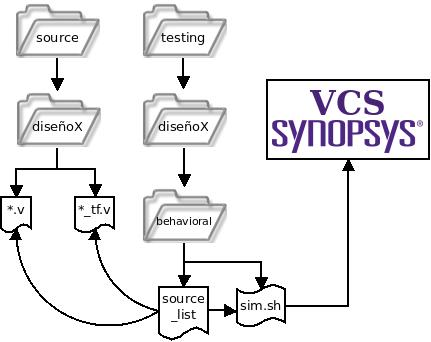
\includegraphics[scale=0.7]{beha_sim.jpeg}
\centering
\caption{Estructura del script de simulación por comportamiento. El archivo \textit{source\_list} apunta hacia el RTL, que se ubican en algún subdirectorio de \textit{source}. El script de simulación llama al archivo \textit{source\_list} al invocar al simulador \textit{VCS}}
\label{beha_sim}
\end{figure}

Para la simulación post síntesis se tiene una estructura similar, pero se tienen dos archivos sin extensión, el primero es el archivo que le indica a la herramienta cuales son los archivos necesarios para la precompilación, estos corresponden al archivo de la tecnología que contiene la biblioteca de simulación, el archivo \textit{HDL} con el netlist generado en la síntesis lógica, para efectos de este proyecto archivos \textit{*\_syn\_sim.v}, y dentro de este último debe estar la directiva de anotación de los retardos para ese diseño indicando la ruta del archivo \textit{*.sdf}. Esta directiva puede incluirse de forma manual, editando el archivo del netlist con algún procesador de texto, o se puede hacer de forma programática utilizando comandos de \textit{TCL} en el script de síntesis, naturalmente es más eficiente usar el segundo método.

La simulación post síntesis requiere que el simulador genere un objeto de alto nivel con las celdas estándar, y el comportamiento del retardo de las señales, es por ello que debe ejecutarse la precompilación y la lectura del archivo \textit{*.sdf} con el fin de que en la simulación pueda contemplarse el efecto de los retardos de propagación de las señales. Se genera un nuevo archivo con los retardos \textbf{*.sdf\_c} y este es el que será usado por el simulador. En la figura

\begin{figure}[h]
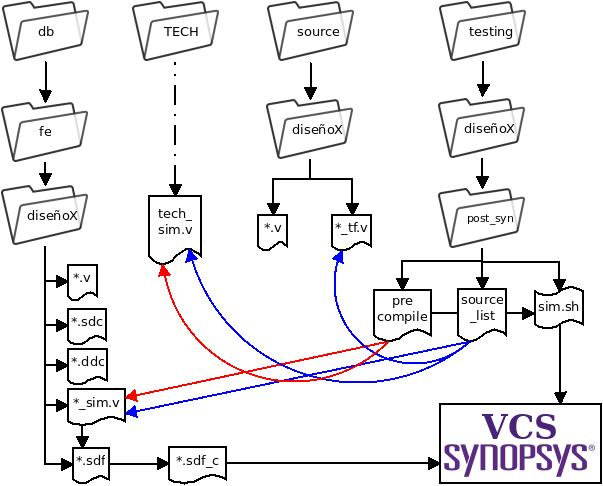
\includegraphics[scale=0.7]{post_syn_sim.jpeg}
\centering
\caption{Estructura del script de simulación post síntesis. El archivo \textit{precompile}, apunta a la biblioteca de simulación y al netlist, eñ \textit{source\_list} apunta hacia el netlist, el código de estímulo, y la biblioteca de simulación. El script de bash, invoca a la herramienta de simulación, realizando primero la precompilación y luego llama al archivo \textit{source\_list} para realizar la simulación}
\label{psyn_sim}
\end{figure}

\section{Scripts de Back End}
\label{sec:phy_s}
\subsection{Script de implementación o síntesis física}
Las herramientas de \textit{Synopsys} siguen un patrón similar en la ejecución de los flujos de síntesis. Nuevamente, conviene tener variables relativas hacia los directorios clave para que la implementación pueda ser ejecutada sin importar la ruta absoluta hacia los directorios. Además se deben definir las variables nativas de la herramienta que garantizan que el flujo será exitoso, tal como los punteros e identificadores hacia las bibliotecas.

Es posible iniciar la implementación de diversas maneras, en el caso del flujo propuesto en este trabajo comienza definiendo las variables principales para la celda física. En el entorno físico de \textit{Synopsys}, la base de datos que contienen la información de la celda, o las celdas físicas se llaman \textit{Milkyway}.

Antes de abrir o crear una base de datos o biblioteca \textit{Milkyway} se deben definir ciertos parámetros y aportarle a la herramienta información importante para la implementación. Esta información corresponde principalmente al nombre de las redes de alimentación y los coeficientes de tiempo de la tecnología, al hablar de coeficientes de tiempo, se refiere a los retardos por efectos parasíticos, que en esencia son los efectos capacitivos y resistivos de los puertos de los transistores \textbf{(Coeficientes RC)} y por lo tanto los \textbf{taus}\footnote{Recordar que "Tau" ($\tau$) corresponde a la constante de carga de una red capacitiva en un circuito eléctrico} de los puertos entrada y salida de cada celda estándar en la tecnología.

Los archivos que contienen la información de los coeficientes se llaman \textit{TLUPlus}, su formato consiste en una base de datos binarios tabulados. Esta información es fundamental en la extracción de los efectos de retardo debido a las parasitancias propias de la tecnología \textit{CMOS}. Si estos no son especificados no se podrá habilitar la "extracción RC" y tener estimaciones de retardo, y consumo dinámico más precisas que serán necesarias para un analisis más exhaustivo con las herramientas \textbf{Primetime} y \textbf{HSpice}.

Una vez se hayan definido los archivos \textit{TLUPlus} y demás parámetros para la celda \textit{Milkyway}, se puede abrir o crear la biblioteca. En este punto es posible tomar diversos caminos para resolver un diseño. Idealmente es posible generar un único diseño jerárquico donde existe una única base de datos, y los subdiseños pueden ser implementados como celdas dentro de la base de datos general del proyecto, así se puede y resolviendo el diseño desde una estrategia que en la jerga del diseño de software se conoce como \textbf{"BottomUp"}. 

Existe otra posibilidad en la que se pueden generar bibliotecas \textit{Milkyway} para cada subdiseño del proyecto principal y al final se exporta una celda con la información del diseño y se usa como una nueva celda estándar, en un diseño futuro (archivo de extensión \textbf{DEF}); sin embargo, aún no ha sido posible determinar la metodología exacta con la que \textit{IC-Compiler} realiza el manejo de los \textit{"Hard-Macros"}.

Es probable que no sea posible terminar un diseño en un único intento, es por ello que el script que se muestra, tiene una bloque condicional el cual se encarga de buscar el archivo \textit{Milkyway} que contiene la información de la celda o el diseño que interesa trabajar. Este condicional evalúa si la base de datos (.mw) existe. Con esa premisa se toma la decisión de abrir la base de datos o en su defecto crearla.

En el caso de que la base de datos exista y se deba abrir alguna celda en particular, conviene dejar el script principal o de inicialización del diseño hasta aquí. A partir de este punto el diseñador tiene múltiples caminos para decidir que hacer con su diseño y no hay una única ruta posible. En este punto es posible invocar múltiples para realizar tareas como evaluación de reglas DRC, análisis de sincronía de señales, re-enrutado selectivo, re-estructuración del colocado de las celdas, optimización de enrutado de acuerdo con criterios de área, potencia, o sincronía, entre muchas otras opciones.

Siguiendo el flujo del diagrama, y asumiendo que se trabaja con un proyecto nuevo, lo que procede es ejecutar el script que importa el diseño. Hay 2 formas principales para cargar un diseño, leyendo un archivo "GL" (HDL a nivel de compuertas) o leyendo un archivo ".ddc", ambos le indican a la herramienta que mediante la base de datos de las celdas estándar de la tecnología se importen las celdas físicas necesarias para iniciar el layout.

La importación del diseño suele involucrar los siguientes procesos: lectura del archivo fuente, la vinculación que resuelve las referencias del diseño y establece la jerarquía de los módulos, luego se desencadena el proceso de remover las celdas multiplicativas instanciadas de la biblioteca jerárquica, esto significa que se genera un nuevo bloque jerárquico que abstrae todas las jerarquías de las instancias y las unifica en una celda. Por su puesto todos estos pasos pueden hacerse por separado, pero la herramienta al importar un diseño los hace de forma automática.

\subsubsection{Floorplan}

Luego de invocar las celdas físicas, la herramienta provee una nueva ventana para visualizar la evolución del layout del diseño. Se procede a definir el floorplan (plano del circuito), esto corresponde a las dimensiones del dado (die o dice). Existen varias formas para establecer un floorplan, que siempre será un rectángulo ya que es la geometría que permite maximizar el aprovechamiento del área al usar celdas con formas de cuadriláteros.

Valiéndose del reporte de área generado en la síntesis lógica y mediante un par de ecuaciones cuadráticas simples, es posible extrapolar las dimensiones del floorplan, habrá que considerar que tan simétrico conviene hacer el espacio o si otra relación de tamaño permite una mejor distribución de las celdas y un diseño más compacto. El diseñador deberá contemplar un presupuesto extra en las dimensiones para el enrutado general, y garantizar un espaciado suficiente para evitar problemas de congestión y demás "DRCs". Además se debe contemplar un margen para puertos de entrada/salida (I/O) y los anillos de alimentación de los cuales se hablará más adelante.

Generar el floorplan de forma manual, y de una forma correcta responde más a la experiencia y la habilidad del diseñador para realizar un buen \textit{ansatz}. Típicamente se deben hacer unas cuantas iteraciones para encontrar el mejor tamaño y relación de aspecto del floorplan. La herramienta permite usar otras metodología para establecer el floorplan, la forma más cómoda que ofrece la herramienta es proveer la relación de aspecto, los margenes desde los puertos I/O hacia el área de colocado, y finalmente el porcentaje del área utilizable para el colocamiento de las celdas, entre más bajo sea este valor, menos probable será enfrentar problemas de congestión y por lo tanto más fácil conseguir un enrutado completo y funcional, pero esto implica que se desaprovecha un porcentaje considerable de área.

Una vez que se haya definido el floorplan se procede a colocar la celdas y a legalizar el colocado, que corresponde a que la herramienta 
efectúe un analisis de posibles conflictos debido a la ubicación de las celdas, así se reubican las celdas estándar del diseño, para evitar cualquier conflicto que se pueda encontrar debido a la colocación de las celdas.

Como ya se mencionó, si se establece un diseño jerárquico, y ya se ha logrado conseguir la síntesis física de los subdiseños que componen el proyecto actual, es posible cargar la información de estas macroceldas ya generadas y tenerlas como premisa para el colocado y enrutado de la nueva macrocelda, esto se logra al crear \textbf{plan\_groups}.

Los "plan\_groups" son áreas restringidas para que las celdas asociadas a una macrocelda se coloquen en una región específica, la colocación de las celdas se hacen a groso modo. Si existen celdas o diseños ya implementados la herramienta puede abstraer el colocamiento que se definió previamente para ese subdiseño y usarlo como punto de partida para agilizar el colocamiento del nuevo diseño, suele complementarse con la lectura de archivos de restricciones que definen el colocado usado para los subdiseños.

\subsubsection{Power Plan}

Una vez que se define la ubicación de las celdas estándar del diseño, se procede a generar el esquema de distribución de la red de alimentación del circuito, existen varias metodologías, exponerlas todas, analizar y discutir sus propiedades está por encima del alcance de este trabajo.

La metodología de distribución de potencia escogida corresponde a un arreglo tipo malla, donde se definen anillos de las redes de alimentación. Mediante un arreglo simétrico de rieles paralelos vertical y horizontalmente, se distribuyen las señales de alimentación en toda el área del dado. Definir una distribución adecuada de la malla de potencia, es laborioso e iterativo, nuevamente depende de que tan bueno sea un ingeniero realizando \textit{ansatz}. Posteriormente cuando se realice la extracción y simulación eléctrica se desvelará si la distribución de potencia cumple con el presupuesto de potencia establecido.

Una distribución de potencia puede diseñarse de forma minuciosa considerando, ecuaciones asociadas a la caída de tensión por perdidas resistivas en el alambrado, fenómenos como la electromigración, radiación, etc. Esta representa una tarea ardua y laboriosa a nivel matemático, usualmente se deberá recurrir a los manuales de descripción física del proceso de integración, además el diseñador deberá tener conocimientos profundos en el área de electromagnetismo a microescala.

Tener un departamento consagrado a la caracterización y diseño para la distribución de potencia en un chip, es más propio de una metodología de diseño \textit{full\_custom}. Para un diseño \textit{semi\_custom} carece de sentido realizar un proceso tan laborioso. Típicamente se usan las herramientas de estimación de alambrado en función al \textbf{IRDrop}, esta abreviación se asocia a las pérdidas de potencia, debido a la disipación resistiva del conductor y electromigración principalmente.

En tecnologías relativamente antiguas (32nm y superiores), que ya han sido altamente depuradas, suele ser recomendable usar las aplicaciones para acelerar el diseño, provista en las herramientas de síntesis. En este caso la aplicación realiza un análisis de la potencia consumida por cada instancia, la aplicación usa el mismo motor que se usa para generar los reportes de potencia, y de acuerdo a las restricciones de diseño definidas en la síntesis lógica, como el factor de actividad, la probabilidad de conmutación, etc, se define un valor estimado del consumo del diseño actual.

Con el valor de potencia necesaria, que ha sido estimado por la herramienta, algunas configuraciones definidas por el usuario, y la información que la biblioteca de la tecnología, la herramienta elabora una propuesta para distribuir las redes de alimentación en el dado.

Al decir que el usuario debe proveer configuraciones se refiere a la tensión gobal del diseño, identificar los metales que serán usados en la red de alimentación, además de sus respectivas propiedades (ancho máximo y mínimo), cantidad máxima y mínima de rieles, entre otras. Cabe destacar que el diseñador deberá proveerle a la herramienta algún medio de conexión, como pueden ser puertos virtuales a "VDD y VSS", sin ellos la herramienta no ejecutará adecuadamente el acelerador de diseño.

En este punto la herramienta presenta gráficamente un arreglo tipo malla, con la propuesta básica de la distribución de potencia. Esta propuesta le permite al diseñador evaluar varias circunstancias relevantes para decidir como proceder a continuación. Por ejemplo, identificar un área donde se concentra un consumo excesivo, podría implicar una reestructuración del colocamiento de las celdas estándar, y así evitar posibles {focos calóricos}\footnote{En la termodinámica se define un foco calórico como un ente que es capaz de intercambiar calor, idealmente, sin que su temperatura se vea afectadas, es decir tendría una disipación térmica continua o constante  \cite{villalobos30entropia}. En el contexto presentado, si un chip presenta una temperatura muy elevada en un sector, podría causar daños a los elementos de la zona, y en casos muy extremos alterar el funcionamiento de los dispositivos, causando problemas como metaestabilidad, pues debido a la naturaleza de los semiconductores, una variaciones en la temperatura puede y causa variación en la mobilidad de los portadores, desencadenando muchos otros fenómenos, que están fuera de la visión de este trabajo.} que puedan comprometer el desempeño del chip una vez fabricado. Es por ello que las bibliotecas manejan condiciones de esquina, no se profundizará en este tema; sin embargo, hay múltiples fenómenos físicos que deben ser considerados y la herramienta le facilita al diseñador tomar de decisiones de acuerdo con los escenarios que se van presentando.

Una vez que el diseñador se siente satisfecho con el \textit{PowerPlan}, se encomienda a la herramienta su implementación, y posteriormente se deben remover los \textit{pads} virtuales que fueron usados para crear el \textit{PowerPlan}. Conviene entonces pre-enrutar la alimentación de las celdas estándar, y generar pads virtuales para efectuar el análisis de potencia a posteriori. Naturalmente la creación e implementación de la distribución de potencia del chip es iterativa y aunque la herramienta facilita su desarrollo, es posible que cuando se efectué un análisis eléctrico, se encuentren deficiencias en la misma, y consecuentemente deba reformarse el \textit{PowerPlan}.

\subsubsection{Enrutamiento y conexión global}

Una vez fueron definidos e implementados el \textit{FloorPlan} y el \textit{PowerPlan} faltaría conectar el resto de dispositivos para obtener el funcionamiento esperado del diseño. A este proceso se le conoce como enrutado (\textit{Routing}). Antes de iniciar el enrutamiento deben definirse algunas restricciones de diseño importantes, como las restricciones sobre el árbol de reloj, reglas de antena, y las restricciones sobre el enrutado global.

\subsubsection*{Árbol de reloj}

Respecto al árbol de reloj se consideraron los siguientes aspectos:

\begin{itemize}
\item Identificador del nombre del reloj.
\item Inserción de celdas frontera cercanas a los puertos de reloj para el diseño basado en jerarquía de bloques.
\item OCV\_Clustering, este atributo permite mejorar la distribución del reloj a través de ramas de registros.
\item Permitir la re-ubicación y el re-dimensionamiento de las compuertas y \textit{búfers} para optimizar la síntesis del árbol de reloj.

Muchos de estos atributos funcionan en conjunto con las restricciones definidas en el proceso de síntesis lógica, como lo son la incertidumbre, o la latencia del reloj, también el netlist generado es de importancia pues con base en este, se le encomienda a la herramienta implementar el árbol de reloj.
\end{itemize}

\subsubsection*{Reglas de antena}

Sobre las reglas de antena, consiste en específicar una serie de atributos avanzados que se almacenaran en la base de datos (biblioteca) \textit{Milkyway} y que permite la inserción de diodos entre el enrutado.

Incluir las reglas de antena, y por lo tanto la inserción de diodos en el enrutado tiene una gran relevancia en el éxito de la fabricación del chip. Una capa delgada en la compuerta de un transistor puede ser fácilmente dañada por una descarga electrostática. En los procesos de múltiples metales, los cables entre capas suelen acumular carga electrostática, esta acumulación de carga electrostática recibe el nombre de \textbf{Antena de acumulación de carga} o simplemente \textbf{Antena}.

El problema únicamente se presenta en la fabricación del chip cuando las conexiones entre capas están incompletas y no existen caminos de descarga disponibles a través de las terminales de fuente, y drenaje del transistor, el problema tiene una mayor probabilidad de presentarse cuando un cable con un área considerable se conecta a un transistor cuya compuerta tiene un área menor.

La herramienta previene los problemas de antena, verificando la entrada de cada celda\footnote{En esencia la herramienta comprueba las conexiones entre el metal de los cables y las compuertas de los transistores de entrada de las celdas}, si se determina una relación  de áreas propensa a un antena entonces la herramienta colocará un diodo de protección para desviar una posible descarga electrostática.

La definición de las reglas de antena está intrínsecamente relacionada al proceso de fabricación y el radio entre el área del cable y la compuerta lo define el proveedor de la tecnología.

Para considerar inserción de diodos y evitar los efectos de antena se establecieron los siguientes criterios:

\begin{itemize}
\item Definición de especificaciones particulares para cada capa de metal y uso de área poligonal.
\item Protección de diodo limitada, esto considerando que si mas de un diodo es necesario para conectar a una antena se colocará un diodo que abarque el efecto total de todas las relaciones de área asociadas a la razón de área entre esa antena y las compuertas conectadas a ella. Es decir se colocará un único diodo capaz de manejar el peor escenario entre la antena y todas la compuertas asociadas a ella.
\item Razón de metal: Especifica la máxima relación permitida entre las áreas del metal y la compuerta. Esto puede considerarse como una condición para considerar si la relación entre un metal y una compuerta amerita colocar un diodo, relaciones excesivas indican un enrutado deficiente y por lo tanto deberá iterarse en este proceso.
\item Radio de corte: Especifica la máxima relación permitida entre las vías entre capas (metales) y las compuertas de los transistores. Al igual que el parámetro anterior permite evaluar la calidad del enrutado.
\item Radio de diodo: Está relacionado con la protección de diodo limitada, aquí se definen las posibles relaciones entre una antena y todas las compuertas asociadas a ella.
\end{itemize}

Los atributos de las reglas de antena los establece el fabricante y la mayoría de los atributos pueden encontrarse en el manual de la tecnología. Los atributos presentados, responden a la información que aporta el manual y al criterio técnico del Dr. Rodríguez.

\subsubsection*{Enrutado global}

La configuración de la herramienta de enrutado (\textit{Zroute}) de \textit{ICC-Compiler} se divide en 4 categorías, configuraciones comúnes, globales, detalladas y de rieles.

En las configuraciones comúnes tenemos, obedecer las restricciones de enrutado, propias de los plan-groups definidos en la etapa de floorplan y que en el enrutado global sean respetadas.

En las configuraciones detalladas, tenemos la inclusión de las reglas de antena, la referencia a los diodos que se utilizaran, y que estos sean considerados durante el enrutado así también como configuraciones por defecto del tamaño de las compuertas (de los transistores), la razón por defecto de la protección de los diodos y emplear un esfuerzo alto para que el enrutado sea convergente con las reglas de diseño.

En las configuraciones globales se establecen condiciones que afectan a todos los comandos que realizan el enrutamiento global. Las configuraciones principales corresponden a enfocar el enrutado para cumplir las especificaciones de sincronía y usar un esfuerzo alto en ello. Finalmente se tienen las configuraciones de enrutamiento asociadas a los rieles que básicamente tiene 2 metodos de optimización, enfocado a la sincronización o al \textit{crosstalk}, la opción escogida corresponde a la de sincronización.

Existe una configuración adicional y corresponde a la estrategia de optimización de los búfers, un esfuerzo medio a bajo se considera adecuado para el enrutamiento, ya que entre más alta sea configurada esta restricción, mayor será la optimización de los búfers, por lo tanto se puede ver afectado el \textit{fanout} de las funciones, aunque permita mejorar la sincronía.

De todos los procesos descritos hasta el momento, podría decirse que el enrutado es el que presenta el mayor empirismo. No obstante a los algoritmos de enrutamiento que presenta la herramienta, cuando se tienen diseños considerablemente complejos muy probablemente la herramienta no será capaz de implementar de forma exitosa todas las interconexiones cumpliendo con las expectativas de sincronización y reglas de diseño en una única ejecución.

Es por ello que en esta etapa se presenta la mayor iteratividad, pues el enrutado debe cumplir con las reglas de diseño propias de la tecnología, las restricciones de implementación que define el diseñador, las reglas de antena, que aunque forman parte de las reglas de diseño, se consideran aparte pues tienen más que ver con el proceso de fabricación que con la tecnología en sí, y fundamentalmente deben cumplirse las expectativas de sincronización.

Tener un enrutado que satisfaga todas las consideraciones anteriores no es fácil por lo que se debe iterar muchas veces este proceso. No hay una secuencia definida para lograr conseguir un enrutado satisfactorio, y cada vez que se optimiza el enrutado, ya sea de forma focalizada para corregir los errores de diseño, errores eléctricos, reglas de antena, sincroná u otro aspecto, se debe comprobar que todas las consideraciones del diseño se cumplen y son satisfactorias.

Cuando se tiene un enrutado satisfactorio se procede a insertar las celdas de relleno y el metalizado de relleno (para este caso celdas sin metales). Los primeros rellenan los espacios vacíos en las filas de colocación de celdas con celdas estándar de relleno. Los últimos se encargan de rellenar los espacios causados por una densidad insuficiente de metal en las capas de los interconexión, se usan cables de relleno, sin conexiones o conectados a tierra para alcanzar las reglas asociadas a la densidad de los metales.

Finalmente queda exportar los reportes y generar los archivos de salida. Respecto a los reportes se genera información congruente con lo expuesto en la sección anterior sobre la síntesis lógica (sección \ref{script_syn}), así que no se ahondará de nuevo en ello.

Los archivos de salida generados son similares a los de la síntesis lógica, nuevamente tenemos un código \textit{HDL} (donde se replica uno para simulación) que contiene el "gate-level-netlist" \textit{GLN} del diseño implementado, un archivo con extensión \textbf{.sdf} con la información de los retardos entre las señales, que es más preciso al generado en la síntesis lógica pues contempla el efecto del cableado, con un modelo muy cercano al real.

Otro archivo de gran importancia corresponde a los archivos con extensión \textbf{.spef} para esto es necesario ejecutar la extracción de los efectos \textit{RC} es decir los retardos parasíticos, el cual le indica a la herramienta que efectué un análisis de retardos usando el modelo de Elmore \cite{book:weste2005} para lo anterior es necesario haber definido los archivos \textit{TLUPlus} que se mencionaron anteriormente.

Un archivo \textbf{.spef} es una lista con información de las parasitancias relativas a las celdas usadas en la implementación del diseño y le permiten a herramientas como \textit{PrimeTime} hacer un modelado más preciso de los tiempos de sincronización que puede ofrecer el analizador del \textit{IC-Compiler}. Se generan archivos para condiciones mínimas y/o máximas si se han definido los escenarios en el diseño, esto último se relaciona con las condiciones esquina que se abstraen de la biblioteca de la tecnología.

Los últimos archivos de salida relevantes para el flujo corresponde al archivo \textbf{.def} y el \textbf{GDS}, ambos consisten en compendios de la información física del diseño, incluyendo información del \textit{layout}, el \textit{netlist} y las restricciones de diseño. La herramienta permite exportar un archivo con toda o alguna de la información del diseño, por ejemplo podría generarse un archiv \textit{.def} únicamente con la información de las vías. El archivo \textbf{GDS} es corresponde al formato estándar con el que los que se intercambia información con el fabricante, este archivo contiene toda la información necesaria para el desarrollo de las máscaras del proceso de diseño, así también como detalles particulares del proceso de fabricación. En este proyecto no fue necesario generar este archivo ya que el trabajo de integración no está completo.La figura \ref{fig:phy_script} resume lo expuesto en este apartado mediante un diagrama de flujo.

\begin{figure}[ht]
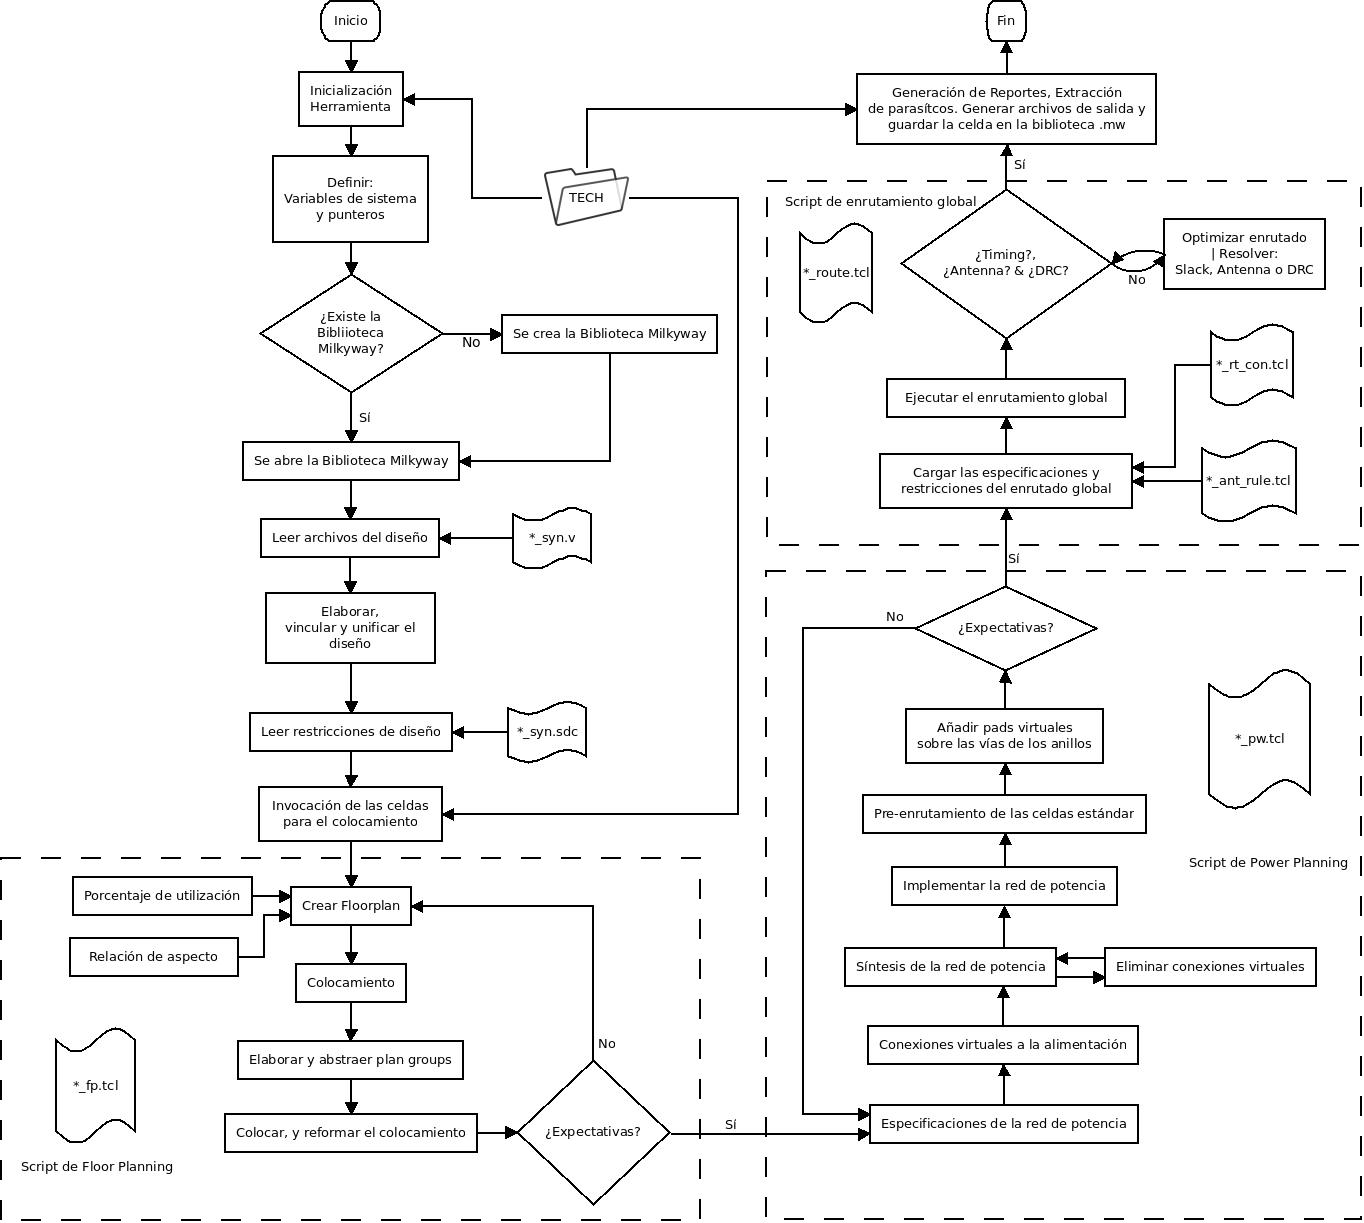
\includegraphics[width=\textwidth]{phy_syn.jpeg}
\centering
\caption{Diagrama de flujo que expone el proceso genérico de la implementación física en la herramienta \textit{IC Compiler}}
\label{fig:phy_script}
\end{figure}

\subsection{Script de simulación física: evaluación post implementación}

Al igual que en el proceso de síntesis es posible determinar la calidad de la implementación mediante el análisis de los reportes, y aunque hacer esto es importante, es necesario validar la funcionalidad del circuito mediante simulaciones \textit{Post-Place\&Route}.

El proceso no se detallará pues sigue la misma estructura que lo expuesto para la simulación post síntesis, en la sección \ref{sec:log_sim} y las diferencias fundamentales consisten en los punteros hacia los archivos fuente para la simulación. Lo cual pueda apreciarse claramente en la figura \ref{fig:phy_sim}.

\begin{figure}[ht]
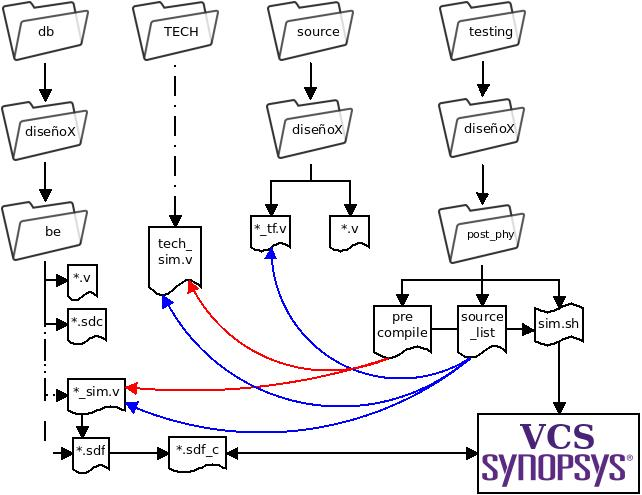
\includegraphics[scale=0.65]{post_phy_sim.jpeg}
\centering
\caption{Estructura del script de bash para la simulación post implementación}
\label{fig:phy_sim}
\end{figure}

\subsection{Script de Análisis de Sincronización Estática STA}
\label{sec:STA}

En esta sección se expone como se incorpora la herramienta \textit{PrimeTime} para evaluar si el diseño cumple las expectativas de sincronización de señales a la velocidad establecida en el diseño.

\textit{PrimeTime} es una herramienta que puede usarse tanto para evaluar un diseño post síntesis lógica como uno post implementación física. En el entorno mostrado en este documento se utiliza con mayor relevancia en la parte de \textit{BackEnd} del flujo pues sus resultados son más concluyentes, y es por ello que la herramienta es mencionada hasta esta sección; no obstante, puede incluirse como una etapa complementaria al flujo de \textit{FrontEnd}

\begin{figure}[ht]
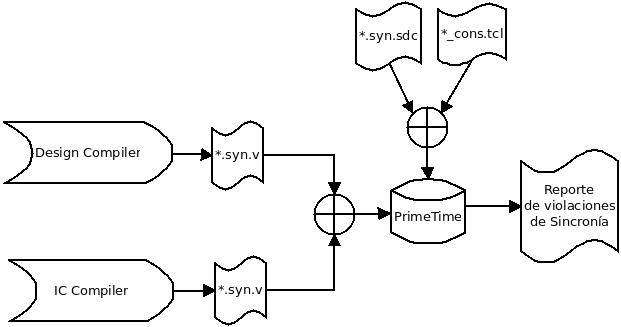
\includegraphics[scale=0.65]{Back_End_STA.jpeg}
\caption{Diagrama de flujo del análsis de sincronización estático}
\label{fig:staflow}
\end{figure}

Como se puede apreciar en la figura \ref{fig:staflow} el flujo de esta herramienta es bastante simple, para la misma se ha desarrollado un pequeño script, en este, como en todos los scripts mostrados hasta el momento, lo principal es inicializar la herramienta, definiendo los punteros hacia los archivos fuente y la biblioteca de la tecnología.

Luego de inicializar la herramienta se cargan los archivos fuente que consisten en: el archivo verilog con el \textit{GLN} implementado, el archivo \textit{SDF} con la información de los retardos de propagación a través del \textit{GLN}, el archivo \textit{SDC} con las restricciones de diseño de \textit{Synopsys} (principalmente las de sincronización), y finalmente el archivo \textit{SPEF} para incluir el efecto de las parasitancias en el análisis. También se pueden incluir otros archivos para realizar otros tipos de análisis como son archivos \textit{SAIF} que es un archivo que indica el factor de actividad de las celdas. De igual manera se puede estimular el diseño con otro conjunto de restricciones, estas corresponden con la misma sintaxis usada en el script de \textit{TCL} para definir las restricciones en la síntesis lógica (*\_cons.tcl).

Debido a que los diseños grandes y complejos presentan una enorme cantidad de restricciones, es necesario efectuar análisis multimodales y multiesquina\footnote{Multiesquina: Traducción literal de multicorner para referirse a que se evaluaran todas las condiciones esquina individualmente} \textit{PrimeTime} permite generar reportes enfocados a escenarios particures de sincronización. Ya sea para evaluar si el diseño cumple con las restricciones de diseño específicadas en una esquina o esquinas determinadas. \textit{PrimeTime} también permite hacer un análisis gráfico, y generar recomendaciones para alcanzar las restricciones de sincronización definidas; sin embargo, adentrar tan profundo en la herramienta está más allá del objetivo de este trabajo.

\begin{figure}[ht]
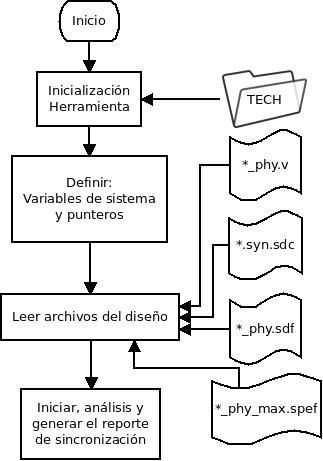
\includegraphics[scale=0.65]{phy_sta.jpeg}
\centering
\caption{Diagrama de flujo del script para un análisis básico de STA en la herramienta PrimeTime de Synopsys.}
\label{fig:stascript}
\end{figure}

El flujo de análisis expuesto en la figura \ref{fig:stascript}, expone un uso relativamente simple de la herramienta, generando un análisis sobre los 3 criterios más relevantes, retardos de entradas a registros, retardos entre registros y retardos de registros a salidas. Para los diseños trabajados en este proyecto, se considera una única condición de esquina, la cual corresponde a los valores típicos de retraso en las señales, una de tensión de 1.2v para las celdas estándar de la tecnología y a temperatura ambiental ($25^{\circ}C$). Estas condiciones se definen al inicializar la herramienta y cargar la biblioteca de la tecnología.

Los reportes generados usan motores similares a los que generan el análisis en las herramientas de síntesis; sin embargo, son más robustos en términos de profundidad y variedad en el análisis. Herramientas como \textit{Design Compiler} y \textit{IC Compiler} usan un modelado dinámico del diseño, valiéndose del peor escenario de propagación de señales, determinado mediante el modelo de Elmore. \textit{PrimeTime} permite usar modelos estáticos y es capaz de analizar distintos escenarios y estimular el diseño de diversas formas, para así evaluar el desempeño de la propagación de señales en distintos bloques de lógica, puramente combinacional, registros, puertos y/o distintas combinaciones de todos ellos.

\section{Script de síntesis de IP Cores y bibliotecas autónomas}
\label{sec:ip_syn}
Este apartado corresponde a una particularidad en el flujo de diseño digital propuesto, ya que no todos los diseños requieren incluir \textit{IPCores}\footnote{Un IPCore, o bloque de propiedad intelectual consiste en un módulo que no ofrece información sobre como es su arquitectura interna. Y su representación consiste en una caja negra. Esto con el fin de proteger la propiedad intelectual}, y la inclusión de los programas necesarios para su inclusión, irrumpe en la regularidad de la estructura de directorios definida anteriormente (ver inicio del capitulo \ref{ch:scripting}).

El flujo del diseño de las \textit{IP Cores}  requiere de 3 herramientas extra, la primera y principal corresponde al sintetizador de memorias de la tecnología utilizada, en este caso corresponde al software para la generación de : Artisan ARM Physical IP. Esta herramienta (Artisan) es un generador de \textit{IP Cores} para celdas de memorias (SRAM y ROM) del proceso IBM CMRF8SF-RVT, que es el proceso usado en este trabajo. La herramienta puede ser invocada a través de scripts, aunque también cuenta con una interfaz gráfica, bastante amigable.

Las 2 herramientas extra mencionadas pertenecen al conjunto de softwares de \textit{Synopsys}, y son el \textit{Library\_Compiler} y \textit{Milkyway}. El primero es necesario para definir una biblioteca lógica dedicada a los \textit{IPCores} y que el bloque SRAM generado pueda ser instanciado en el diseño y consecuente abstraído como un \textit{hardblock} en los procesos de síntesis. \textit{Milkyway} sirve como complemento para generar las bibliotecas físicas de las celdas.

No se expondrá mucho sobre el \textit{Library\_Compiler}, pues su uso es muy simple, y muy puntual. Esta herramienta es necesaria ya que al ejecutar Artisan, los productos de la síntesis de un \textit{IPCore} son archivos:

\begin{itemize}
\item Verilog, con el modelo \textit{GLN} para instanciar la celda generada. Algo equivalente a lo que se obtendría efectuando una síntesis lógica en \textit{DesignCompiler}.
\item dat, que es una tabla \textit{ASCII} con un resumen de la información geométrica y eléctrica de la celda.
\item PostScript, que es una pequeña hoja de datos con diagramas de sincronía e información sobre los puertos en formato ".ps".
\item VCLEF, este archivo contiene la información de la distribución de pads, diodos y metales para el enrutado (interconexión) y conexión externa en la celda.
\item CLF, es un archivo útil principalmente para las herramientas de \textit{Cadence} que es otro provedor de herramientas para diseño VLSI.  Sin embargo, los \textit{foundries} suelen solicitar este archivo por motivos de estandarización, así que conviene conservarlo. Contiene información relacionada con la antenas (Antenna) y los diodos de protección.
\item lib, acrónimo del formato liberty, que es un estándar para definir los parámetros de sincronía y potencia de la celda, así también como la conectividad con el exterior. Este archivo en conjunto al vclef permiten definir la celda física del \textit{IPCore}.
\item data, este es un archivo necesario para ejecutar el análisis \textit{STA} con \textit{PrimeTime}; sin embargo, requiere de una precompilación con un script de \textit{PERL} para generar correctamente el archivo \textit{.sdf}
\end{itemize}

Artisan permite generar más archivos de salida, para otra familia de herramientas como \textit{Cadence} por ejemplo; sin embargo, se han expuesto únicamente aquellos archivos relevantes para el flujo de diseño digital en cuestión, que se desarrolla en \textit{Synopsys}.

Teniendo claro lo anterior, es más fácil comprender cuál es el rol de las herramientas \textit{Library\_Compiler y Milkyway}, pues con ellos se generan las bibliotecas para el flujo.

\textit{Library\_Compiler} traduce la biblioteca en formato \textit{liberty (.lib)} al formato \textit{database (.db)} de \textit{Synopsys} con el fin de poder incluir la celda de memoria generada en el flujo \textit{FrontEnd}, en un diseño en particular. \textit{Milkyway} compila la información de la biblioteca de la tecnología, el archivo \textit{.vclef} y la biblioteca \textit{.db} (generada previamente por el \textit{Library\_Compiler}), para así desarrollar una nueva biblioteca \textit{.mw} que permita incluir la celda de memoria en el flujo \textit{BackEnd}, en un diseño en particular.

Las instrucciones necesarias para compilar la biblioteca en formato \textit{liberty} a una en formato \textit{database} son las siguientes, observe que la palabra library\_name se encuentra entre comillas, en este segmento se debe colocar el nombre de la biblioteca (sin comillas), el cual se definió al usar la herramienta \textit{Artisan}

\begin{lstlisting}[language= tcl, numbers=left, keywordstyle=\color{blue}, commentstyle=\color{mygreen}]
read_lib library.lib
write_lib "library_name" -format db -output library.db
\end{lstlisting}


El script para ejecutar la herramienta \textit{Milkyway} sigue un proceso similar al de la síntesis física. Primero se configuran los punteros y las bibliotecas de la tecnología. Luego se crea o se abre la biblioteca \textit{*.mw}, para incluir las nuevas celdas. Posteriormente al inicializar la biblioteca \textit{Milkyway} se leen los archivos \textit{.vclef}, aquí es importante destacar que la referencia un archivo particular de la tecnología (lefin\_layer\_map.txt) debe hacerse con cuidado. Este archivo contiene alias de los nombres de los metales de la tecnología, sin el es imposible generar de forma exitosa la biblioteca física. Los alias definidos en el archivo lefin\_layer\_map.txt deben ser congruentes con los nombres de los metales de la tecnología, de no ser así, deben ser editados. Este archivo debe incluirse ya que la herramienta \textit{Artisan} nombra de forma diferente a los metales cuando genera los archivos \textit{*.vclef}. Finalmente se leen los archivos \textit{.db} para actualizar la información de los puertos, en términos de la sincronía de las señales, etc. 

Como una consideración final, para mantener la regularidad, localidad y continuidad en los directorios y archivos, que se ha intentado establecer desde el principio, conviene tener una única biblioteca \textit{Milkyways} para los \textit{IP Cores}, así cada nueva macro celda se abstraerá de una única biblioteca auxiliar.

\begin{figure}[ht]
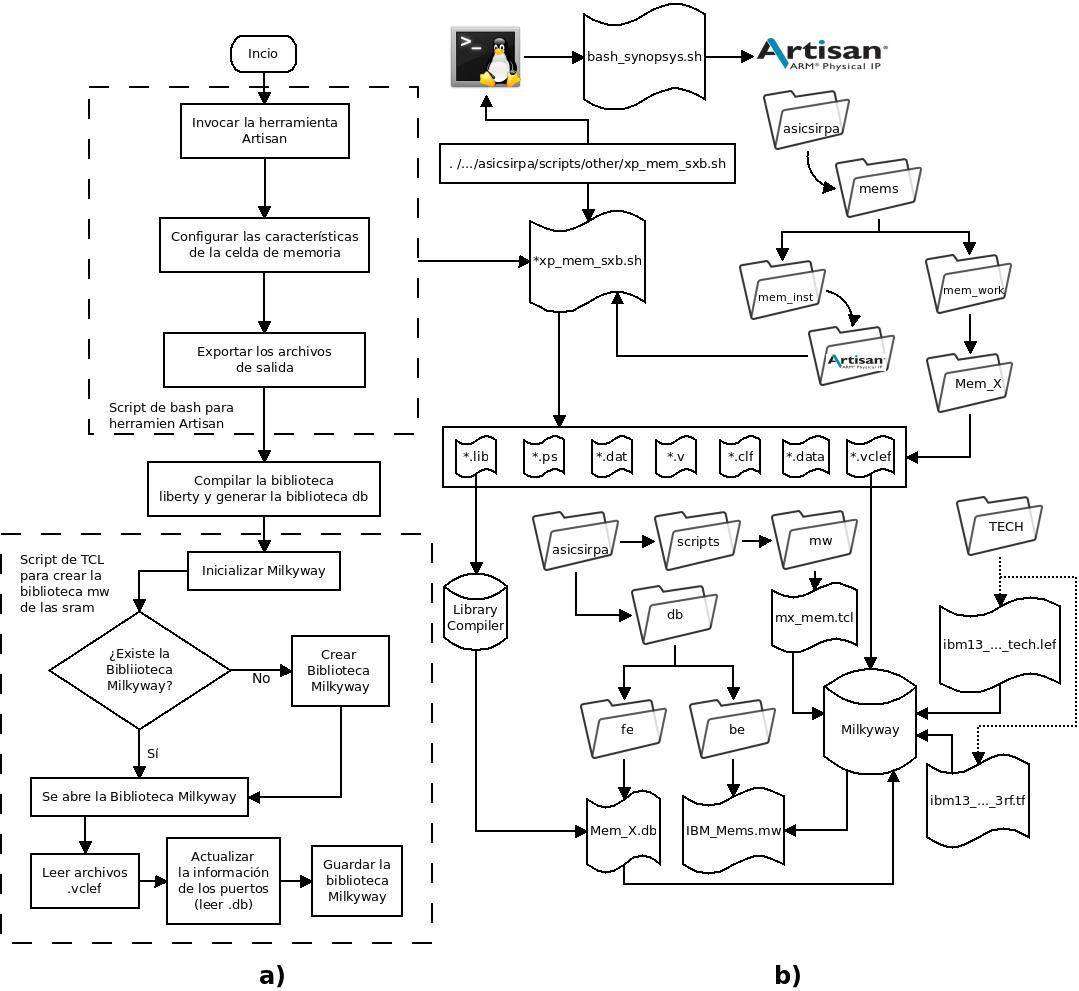
\includegraphics[width=\textwidth]{RAM_Syn.jpeg}
\centering
\caption{a) Diagrama de flujo de la síntesis de los \textit{IP Cores} de memorias SRAM y generación de las bibliotecas autónomas. \newline b) Estructura de directorios y archivos que intervienen en la síntesis de los IPcores de las memorias, herramientas involucradas y los archivos generados.}
\end{figure}

\newpage

\section{Análisis de resultados: Scripting }

En primera instancia cabe destacar que determinar la eficiencia de una estructura de directorios y archivos que pretenden realizar una tarea programática particular, depende de los paradigmas de trabajo individuales o de un equipo de trabajo. Por lo tanto no se puede establecer de forma cuantitativa que tan eficiente es la estructura de scripting que se planteó en este capítulo. En consecuencia este apartado se presenta como un análisis subjetivo y cualitativo del resultado obtenido en la experimentación con las herramientas de \textit{Synopsys} y la integración de un microprocesador \textit{RISC-V} para el proyecto \textit{SiRPA}.

Como se mencionó al inicio del capítulo, la forma en que los directorios y archivos fueron dispuestos responde a tres criterios, regularidad, localidad y continuidad. La estructura mostrada en la figura \ref{directorios} presenta una alta regularidad pues la mayoría de directorios tienen la misma jerarquía. Es continua, pues como puede observarse en las figuras \ref{beha_sim}, \ref{psyn_sim} y \ref{fig:phy_sim}, es posible rastrear los productos de los distintos procesos que afectan a los archivos. Finalmente, cuando un archivo es generado no es necesario, replicarlo en ningún otro directorio, los procesos que lo necesiten a posteriori pueden acceder a ellos mediante punteros, definidos en los scripts de los procesos que los requieran.

Finalmente quisiera declarar que lo expuesto en este capítulo tienen como sustento bibliográfico los manuales y páginas man de las herramientas de \textit{Synopsys}. La temática de la implementación del flujo digital respecto al \textit{Scripting} corresponden a una libre interpretación de la información contenida en estos manuales y las páginas man.








